\section{Networking, Localization, and Data Management Framework for Drone}
\label{networkingsection}
%Navigation, networking, localization

For autonomous drone-based monitoring, the prerequisite is a self-operating framework.
\red{The crucial}
factors that need to be considered for autonomous operation \red{are} speed, safety and data management, \red{which we discuss in the following}.

\subsection{Autonomous Navigation}
In \red{a} known environment, a drone can \textcolor{blue}{operate} avoid\textcolor{blue}{ing} obstacles easily while in an unknown environment, it is difficult to operate \textcolor{blue}{without avoiding obstacles. There has been a good number of researches performed in the area of autonomous navigation for drones}. In \textcolor{blue}{most of} the  case\textcolor{blue}{s}, either the \textcolor{blue}{proposed} system is safe but slow, or the system works fast but unsafe. \red{Most recently,} a system has been implemented that can operate independently in an unknown environment safely \red{while maintaining a good speed}~\cite{tordesillas2019real}. \red{From a drones perspective, the real world can be divided into two parts; (i) the flying zone for the the drone and (ii) outside map area.}
\textcolor{blue}{Tordesillas et al.} have partitioned the flying zone area into 3 spaces~\cite{tordesillas2019faster}, \textcolor{orange}{which is presented in Fig~\ref{autonomous}}.
%\az{Connect these paragraphs}
\textcolor{blue}{The area marked with F}  is known \textcolor{blue}{as} free space which is the instructed space with no construction change. The \textcolor{blue} {area marked with O}  is known \textcolor{blue}{as} occupied space  which can be represented by the change in construction or the intervene of any real-world object such as a bird. \textcolor{blue}{T}he last one is the unknown space (U) that might be required based on the real-world situation.
\begin{figure}[h!]
\centering
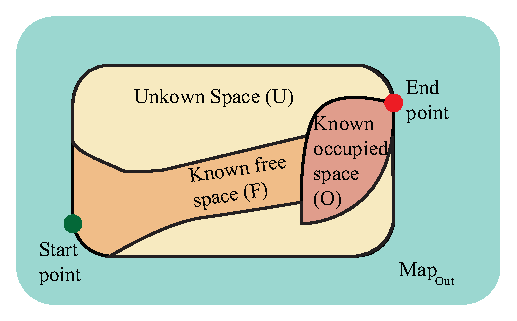
\includegraphics[width=.65\linewidth]{figure/autonomous.eps}
\caption{Flying map with drone perspective.}
\label{autonomous}
\end{figure}


In the proposed system by \todo{system proposed in 1st or 2nd reference? -1st -done}\textcolor{blue}{Liu et al.} in~\cite{liu2017planning}, \textcolor{orange}{has used Jump Point Search (JPS)~\cite{harabor2011online} as an universal planner to find the shortest possible route from the starting point to the ending point.} %Another alternative \textcolor{blue}{technique} is A\(^*\)  but 
JPS not only ensures faster magnitude \textcolor{orange}{of the flight speed} but also guarantees the completeness and \textcolor{blue}{optimality}. \textcolor{orange}{This JPS based hierarchical input control} %\todo{path finding algorithm? -done}
consists of three parts i.e., a part controlled by jerk, a part controlled by velocity, and a part controlled by geometry. By using the map, the collision search for each of the three primitives mentioned above the whole performance can be summarized as follows. If it does not collide, the jerk operated trajectory is treated as collision-free. The velocity-controlled primitive is forced to traverse the JPS solution's paths. Eventually, a no-hit obstacle is confirmed to hit the JPS route. 
% The cost for the planned trajectory is calculated by the following equations.
% $$\text{Cost}=J_{\text{Prim}_{j}}+J_{\text{Prim}_{v}}+J_{\text{Prim}_{d}}$$

% Here, $J_{\text{Prim}_{j}}$ represents jerk-controlled primitive, $J_{\text{Prim}_{v}}$ is combination of multiple primitives regulated by velocity, and $J_{\text{Prim}_{d}}$ is the portion of JPS.

\begin{comment}
Besides, a monocular camera based drone system was proposed, where can operate autonomously in the preceding unknown indoor hallway area, where GPS is not working properly~\cite{padhy2018deep}. They have used the CNN model to reach the goal. Video captured by the camera is fed to the model, then the model takes the decision. The CNN model is designed with 4 convolutional layers and 4 pooling layers. The output of the model is left, right, and straight.
\end{comment}
\red{Alternatively,}
\textcolor{blue}{deep learning based models are also being used to facilitate the autonomous navigation of drone systems from different perspectives. Padhy at el. proposed to use state-of-the-art convolutional neural network (i.e., DenseNet-161) to classify the frames of drone videos captured with monocular camera, based on different directions (i.e., left, right or center) of the GPS-unidentified indoor corridors~\cite{padhy2018deep}. The model was supervisedly trained on the images captured in different indoor corridor environments and evaluated with no-collision ratio and full-flight ratio.}
\textcolor{blue}{Another} deep learning-based network was experimented on a little shaped drone \textcolor{blue}{equipped with optical flow sensor, sonar and Lidar Lite V3}~\cite{smolyanskiy2017toward}.
\textcolor{blue}{The experiments were conducted in} different \textcolor{blue}{challenging} circumstances, e.g., a  relatively straight forest trail with 100 m length, a  zigzag forest path with 6 turns, a 1 km mountainous zigzag forest path, and an open field. Another \textcolor{blue}{proposed} network namely TrailNet is inspired by sResNet-18 \textcolor{blue}{which} is basically a ResNet-18 with batch normalization and shifted Relu \red{activation} instead of Relu \red{activation}~\cite{he2016deep}. %Input of the TrailNet is the image capured by the drone and outputs of the model are view orientation and lateral offset. By using these two output parameters the drone can fly indepnedently. 
\textcolor{blue}{The model classifies the drone images into three categories of view orientation along with three types of lateral offsets.} Besides \textcolor{blue}{of navigation tasks}, they have also implemented safety feature\textcolor{blue}{s} for the drone, e.g., obstacle detection and avoidance~\cite{he2016deep}.

\red{Autonomous drone racing is an exciting area where these navigational techniques are put through the ultimate test.}
In the racing track, a drone \textcolor{blue}{has} to pass though several square gates \textcolor{blue}{without collision}. As all the gates look exactly same, and one gate is \textcolor{blue}{visible} through others, it is a very \textcolor{blue}{difficult} task to \textcolor{blue}{detect} the nearest gate. A \textcolor{blue}{CNN based network named as} ADRNet (Autonoumous Drone Racing Network) was developed \textcolor{blue}{focusing on the autonomous drone racing }~\cite{jung2018perception}. \textcolor{blue}{The proposed model can detect the center of a gate.} \textcolor{blue}{Along with the model results,} line-of-sight guidance algorithm \textcolor{blue}{was incorporated for flight control, to}  develop a drone system, \textcolor{blue}{which} can \textcolor{blue}{complete} a race track. 

\subsection{Safety Features}
In practical life, a drone may encounter unexpected obstacles such as a ball coming toward it, which can cause damage to the drone. Besides, covering 360$^{\circ}$ safety is not only costly but also computation expensive. Therefore, one possible solution is using sonar sensors embedded with the drone. One of the possible solutions is utilizing the Doppler effect~\cite{garg2020enabling}. \red{Given} \textcolor{blue}{a stationary sound source and microphone system as shown in Fig~\ref{safety}, a drone can detect Doppler shift for a nearby moving obstacle coming towards the drone with $v_{\circ}$ speed.} According to the formula \ref{eqn:doppler_effect}, a drone can detect Doppler shift for a nearby moving obstacle coming towards the drone with $v_{\circ}$ speed and an $\theta$ angle with the drone\textcolor{blue}{.}
\begin{equation}
\label{eqn:doppler_effect}
    \Delta f=f_{\circ} \frac{2 v_{\circ} \cos (\theta)}{v}
\end{equation}



%if a sound source with $f_{\circ}$ coming towards an object with a $v_s$ velocity, then the frequency experienced by the object will be $$f=f_{\circ} \frac{v+v_{s}}{v-v_{t}}$$

% Here, $v$ and $v_t$ are the speed of sound and target respectively. However, with a stationary sound source and microphone system as shown in Fig~\ref{safety}, a drone can detect Doppler shift for a nearby moving obstacle coming towards the drone with $v_{\circ}$ speed. According to the theorem, the total Droppler shift will be, $$\Delta f=f_{\circ} \frac{2 v_{\circ}}{v-v_{\circ}}\approx f \frac{2 v_{\circ}}{v} \left[\text{as } v_{\circ}<<v\right]$$

\begin{figure}[h!]
\centering
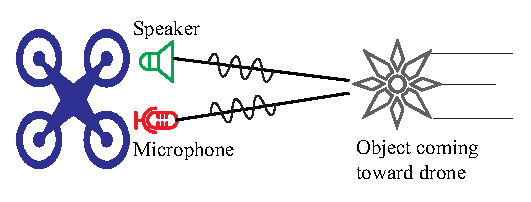
\includegraphics[width=.7\linewidth]{figure/safety.eps}
\caption{Doppler effect on drone.}
\label{safety}
\end{figure}

% Considering the velocity direction, if the moving object makes an $\theta$ angle with the drone, then only the cosine component of the object's velocity will influence the doppler shift. On that case, $$\Delta f=f_{\circ} \frac{2 v_{\circ} \cos (\theta)}{v}$$ 

 However in practice, the doppler shift deviates from the ideal value because of various factors such as environmental drag. Therefore, instead of estimating the Doppler effect, the change of the effect is calculated with respect to $\Delta $ time. As $v_{\circ}$ and $\theta$ are both functions of time, the ratio  \textcolor{blue}{can be expressed by equation \ref{eqn:angle_ratio}.} 
\begin{equation}
\label{eqn:angle_ratio}
   \frac{\Delta f(t+\Delta t)}{\Delta f(t)} \approx \frac{\cos \left[ \theta(t+\Delta t)\right]}{\cos \left[\theta(t)\right]} 
\end{equation}


This angle ratio is the changing rate of radial angle. If the value is constantly one over multiple time segments, then it means an object is coming towards the drone, that might hit it. For other non-constant values, it is safe. Therefore, utilizing this value the drone can improve its safety mechanism and dodge any harmful materials coming towards it.

Another important safety feature is safe landing. A safeUAV-nets has been proposed which make the landing safer for the drone~\cite{marcu2018safeuav}. The main task of this net is to identify the Horizontal area such as a rooftop, plain ground, in other words, a safe landing spot. For this purpose RGB camera has been used. The safeUAV-nets not only predict the safe landing ground but also estimate the depth from the UAV to the ground.

\red{Reinforcement learning-based obstacle avoidance models~\cite{singla2019memory} have also garnered significant attention recently.}
% A reinforcement learning-based obstacle avoidance model was proposed for the drone. 
\red{The authors of~\cite{singla2019memory} have used recurrent neural network and temporal attention as the base of their reinforcement learning framework.}
% The base of this model~\cite{singla2019memory} is the recurrent neural network and temporal attention. 
They have adopted \textcolor{orange}{conditional GAN \cite{isola2017image}}  for depth estimation. Such depth maps are feed to reinforcement with RNN (LSTM) model and the model returns the flight command. The reward function of the learning is designed by taking into account the aerial systems power consumption and the time factor in navigation operations. Though depth \textcolor{orange}{was} predicted from unseen material world images, the output \red{was found to be} noisy.

\subsection{Signal Processing and Data Management}
\red{Drones, often equipped with a number of visual, radar and audio sensors can generate a staggering amount of data in a short amount of time which often needs to stored and processed in small embedded SoCs.}
% One of the major limitations in the field of machine learning is the limited space of an embedded system. 
So, it is important to store data more efficiently and \red{and online data compression is one the most used techniques in such scenarios.}
% One common technique is data compression while recording. 
Motivated by \cite{hitomi2011video}, \red{the authors of }~\cite{kumar2018onboard} \red{employed} imaging methodology to increase the frame rate of a normal off-the-shelf camera by using a silicon liquid crystal to compressively attain video-coded snapshots. Compression is performed out by using coded aperture imaging on a given hyperspectral datacube. For decompression, \textcolor{blue}{t}hey have suggested a sparse recovery algorithm based on a deep neural network to rebuild the datacube from compressively coded snapshots. This form of sparse data acquisition is usually decompressed using sparse recovery algorithms such as orthogonal matching or iterative hard threshold, which is \red{a very} slow process.

Another scheme to increase the working efficiency of the model is data augmentation. 
\red{Authors of~\cite{milz2018aerial}} proposed a \textcolor{orange}{conditional GAN \cite{isola2017image}} based method that can generate sensor data of various kinds, such as camera images or Lidar point clouds.
% The fundamental idea is to use a cGAN \red{[CITE]} and the desired ground truth can be fed to any model as conditional input.
A two-stream CNN technique has been presented that can predict the depth without using any depth sensor~\cite{kouris2018learning}. The network takes consecutive RGB image frames as input and returns the distance of any object from the drone in three directions. The CNN network is trained with a custom dataset where the actual distance from the object to the drone was collected using external HC-SR04 Ultrasonic Sensor and GP2Y0A60SZLF Analog IR Sensor mounted on the drone.